\chapter{STrans 软件使用说明书}\label{manual-strans-ux8f6fux4ef6ux4f7fux7528ux8bf4ux660eux4e66}

\section{文档信息}\label{manual-ux6587ux6863ux4fe1ux606f}

\begin{longtable}[]{@{}
  >{\raggedright\arraybackslash}p{(\linewidth - 2\tabcolsep) * \real{0.5000}}
  >{\raggedright\arraybackslash}p{(\linewidth - 2\tabcolsep) * \real{0.5000}}@{}}
\toprule\noalign{}
\begin{minipage}[b]{\linewidth}\raggedright
项目
\end{minipage} & \begin{minipage}[b]{\linewidth}\raggedright
内容
\end{minipage} \\
\midrule\noalign{}
\endhead
\bottomrule\noalign{}
\endlastfoot
软件名称 & STrans 智慧交通视觉感知与管理系统 \\
文档版本 & V1.0 \\
编制日期 & 2026-07-14 \\
适用对象 & 系统管理员、普通用户、算法工程人员、部署与维护人员 \\
适用范围 & 当前 \texttt{L\allowbreak{}I\allowbreak{}N\allowbreak{}G} 分支及结题交付工作区 \\
配套文档 & \texttt{09-\allowbreak{}系统设计说明书.\allowbreak{}md}、\texttt{06-\allowbreak{}系统测试报告.\allowbreak{}md}、\texttt{10-\allowbreak{}真实数据集识别测试报告.\allowbreak{}md}、M01--M13 模块说明 \\
\end{longtable}

本说明书用于指导 STrans 的安装、启动、日常操作、数据管理、道路建模和故障处置。文中只描述当前仓库已经具备的能力；物理闸机、独立碰撞识别、信号灯识别和完整跨线流量统计不属于当前交付范围。

\section{软件概述}\label{manual-ux8f6fux4ef6ux6982ux8ff0}

STrans 面向智慧交通沙盘场景，将 RTSP/MJPEG 网络流、手机或 USB 摄像头、本地图片和本地录像统一接入计算机端，在本地完成车辆检测与跟踪、车牌识别、白名单判断、道路异常候选检测、道路语义分割和道路空间映射，再通过 React Web 大屏展示实时画面、交通状态和告警。

系统的业务主线为：

\begin{quote}
视频采集 → 模型识别 → 道路分析 → 告警处置 → 历史与证据归档
\end{quote}

主要组成如下：

\begin{longtable}[]{@{}
  >{\raggedright\arraybackslash}p{(\linewidth - 4\tabcolsep) * \real{0.3333}}
  >{\raggedright\arraybackslash}p{(\linewidth - 4\tabcolsep) * \real{0.3333}}
  >{\raggedright\arraybackslash}p{(\linewidth - 4\tabcolsep) * \real{0.3333}}@{}}
\toprule\noalign{}
\begin{minipage}[b]{\linewidth}\raggedright
层次
\end{minipage} & \begin{minipage}[b]{\linewidth}\raggedright
主要组件
\end{minipage} & \begin{minipage}[b]{\linewidth}\raggedright
用途
\end{minipage} \\
\midrule\noalign{}
\endhead
\bottomrule\noalign{}
\endlastfoot
展示层 & React、Vite、HTML5 Canvas & 登录、实时监控、热力图、功能中心、道路建模入口 \\
API 层 & FastAPI & 认证、摄像头、识别、历史、告警、报告和管理接口 \\
视频接入 & CameraHub、VideoStreamService & 多路视频配置、启停、解码、重连和 MJPEG 输出 \\
视觉感知 & LocalModelService、RoadAnomalyService、RoadMaskService & YOLO/ByteTrack、HyperLPR3、异常候选、SegFormer 道路分割 \\
交通分析 & RoadLogicService、AdaptiveModelScheduler & 单应映射、车道/路口归属、拥堵、禁停和资源自适应 \\
数据服务 & AnalysisStore、WhitelistStore、AuthStore & SQLite 历史、告警、证据、白名单、账号和审计 \\
辅助工具 & 道路建模工具、智能报告服务 & 道路拓扑与标定 JSON 生产、监测报告生成与归档 \\
\end{longtable}

\section{运行环境}\label{manual-ux8fd0ux884cux73afux5883}

\subsection{已验证环境}\label{manual-ux5df2ux9a8cux8bc1ux73afux5883}

\begin{longtable}[]{@{}ll@{}}
\toprule\noalign{}
项目 & 已验证配置 \\
\midrule\noalign{}
\endhead
\bottomrule\noalign{}
\endlastfoot
操作系统 & Windows 11，64 位 \\
主项目 Python & Python 3.14.3 \\
PyTorch / CUDA & PyTorch 2.11.0+cu126，CUDA 可用 \\
GPU & NVIDIA GeForce RTX 4050 Laptop GPU，6141 MiB 显存 \\
CPU / 内存 & Intel Core i7-14650HX，16 核 24 线程 / 31.71 GB \\
Node.js / npm & Node.js 24.14.0 / npm 11.12.1 \\
前端浏览器 & Chromium 内核浏览器；已验证 1366×768 和 1920×1080 \\
后端默认地址 & \texttt{http:\allowbreak{}/\allowbreak{}/\allowbreak{}127.\allowbreak{}0.\allowbreak{}0.\allowbreak{}1:\allowbreak{}8000} \\
前端默认地址 & \texttt{http:\allowbreak{}/\allowbreak{}/\allowbreak{}127.\allowbreak{}0.\allowbreak{}0.\allowbreak{}1:\allowbreak{}5173} \\
本地数据库 & SQLite，默认由后端服务管理 \\
\end{longtable}

\subsection{推荐配置}\label{manual-ux63a8ux8350ux914dux7f6e}

\begin{itemize}
\tightlist
\item
  正式识别演示建议使用支持 CUDA 的 NVIDIA GPU，显存不低于 6 GB；
\item
  内存建议 16 GB 以上，并为模型权重和视频缓存保留足够磁盘空间；
\item
  浏览器建议使用当前版本 Chrome、Edge 或 Playwright Chromium；
\item
  本地录像和图片路径应使用当前 Windows 用户可读的绝对路径；
\item
  多路实时视频应优先使用稳定的有线网络，并确保 RTSP/MJPEG 地址从运行主机可访问。
\end{itemize}

\subsection{GPU、CPU 与 Python 环境说明}\label{manual-gpucpu-ux4e0e-python-ux73afux5883ux8bf4ux660e}

系统支持 CUDA 优先、CPU 降级。当前项目 \texttt{.\allowbreak{}venv} 中的 Torch 为 CPU 构建，可用于单元测试和基本功能检查；结题阶段的 65 帧离线评测与前端实时识别均使用 \texttt{C:\allowbreak{}\textbackslash{}\allowbreak{}\allowbreak{}Python314\textbackslash{}\allowbreak{}python.\allowbreak{}exe} 的 CUDA 环境。

同一批 65 帧样本中，CUDA 平均推理耗时为 683.20 ms，CPU 功能预跑为 1158.06 ms，平均耗时下降约 41.0\%。该结果反映当前设备和软件组合下的运行速度，不等同于识别精度提升。更换 GPU、Python、PyTorch、CUDA、模型权重或摄像头后，模型兼容性、时延和少量数值结果可能变化，应重新记录环境并执行回归测试。

\section{安装与部署}\label{manual-ux5b89ux88c5ux4e0eux90e8ux7f72}

\subsection{部署前检查}\label{manual-ux90e8ux7f72ux524dux68c0ux67e5}

\begin{enumerate}
\def\labelenumi{\arabic{enumi}.}
\tightlist
\item
  确认仓库位于可读写目录，路径中不存在受限权限；
\item
  确认 Python、Node.js、包管理器、FFmpeg 和 GPU 驱动可用；
\item
  确认端口 8000、5173 未被其他进程占用；
\item
  确认模型权重、本地视频和 SQLite 数据目录有足够空间；
\item
  正式环境应先设置管理员密码和外部服务密钥，不使用演示配置作为生产配置。
\end{enumerate}

\subsection{后端安装}\label{manual-ux540eux7aefux5b89ux88c5}

在仓库根目录执行：

\begin{Verbatim}[breaklines=true,breakanywhere=true,fontsize=\small,frame=single,framesep=2mm,rulecolor=\color{STransLine}]
cd backend
python -m pip install -r requirements.txt
\end{Verbatim}

若只执行轻量单元测试，可使用项目已有的 CPU 虚拟环境；若要运行正式视觉识别，应确保当前 Python 中 \texttt{torch.\allowbreak{}cuda.\allowbreak{}is\_\allowbreak{}available()} 返回 \texttt{True}，且 PyTorch CUDA 版本与显卡驱动兼容。

后端启动命令：

\begin{Verbatim}[breaklines=true,breakanywhere=true,fontsize=\small,frame=single,framesep=2mm,rulecolor=\color{STransLine}]
cd backend
python -m uvicorn app.main:app --host 127.0.0.1 --port 8000
\end{Verbatim}

启动后先访问 \texttt{http:\allowbreak{}/\allowbreak{}/\allowbreak{}127.\allowbreak{}0.\allowbreak{}0.\allowbreak{}1:\allowbreak{}8000/\allowbreak{}api/\allowbreak{}health} 检查服务状态。模型采用按需加载方式，第一次识别通常包含权重加载和 CUDA 预热开销。

\subsection{前端安装与启动}\label{manual-ux524dux7aefux5b89ux88c5ux4e0eux542fux52a8}

\begin{Verbatim}[breaklines=true,breakanywhere=true,fontsize=\small,frame=single,framesep=2mm,rulecolor=\color{STransLine}]
cd frontend
pnpm install --frozen-lockfile
pnpm dev -- --host 0.0.0.0
\end{Verbatim}

浏览器访问 \texttt{http:\allowbreak{}/\allowbreak{}/\allowbreak{}127.\allowbreak{}0.\allowbreak{}0.\allowbreak{}1:\allowbreak{}5173}。Vite 默认将 API 指向 \texttt{http:\allowbreak{}/\allowbreak{}/\allowbreak{}localhost:\allowbreak{}8000}；如果后端地址不同，应通过前端环境配置调整 \texttt{V\allowbreak{}I\allowbreak{}T\allowbreak{}E\_\allowbreak{}\allowbreak{}A\allowbreak{}P\allowbreak{}I\_\allowbreak{}\allowbreak{}B\allowbreak{}A\allowbreak{}S\allowbreak{}E}。

生产构建命令：

\begin{Verbatim}[breaklines=true,breakanywhere=true,fontsize=\small,frame=single,framesep=2mm,rulecolor=\color{STransLine}]
cd frontend
pnpm build
\end{Verbatim}

构建结果位于 \texttt{frontend/\allowbreak{}dist/\allowbreak{}}，其中包含道路建模静态页面 \texttt{dist/\allowbreak{}road\_\allowbreak{}logic\_\allowbreak{}modeler/\allowbreak{}}。

\subsection{模型与可选服务}\label{manual-ux6a21ux578bux4e0eux53efux9009ux670dux52a1}

\begin{itemize}
\tightlist
\item
  车辆模型、车牌模型和道路分割模型在本地运行；缺失模型可按现有下载逻辑准备，正式演示前应提前下载并完成一次预热；
\item
  SegFormer 道路分割模型位于 \texttt{data/\allowbreak{}models/\allowbreak{}segformer-\allowbreak{}b0-\allowbreak{}cityscapes/\allowbreak{}}，首次准备需要网络和足够磁盘空间；
\item
  智能报告需要管理员配置兼容的 DeepSeek API 地址、模型和密钥。未配置或外部服务不可用时，核心识别链路不受影响；
\item
  远程算法服务是可选能力，未启用时系统使用本地模型；
\item
  道路建模的 RTSP 单帧桥接为本机可选工具，仅监听 \texttt{127.\allowbreak{}0.\allowbreak{}0.\allowbreak{}1:\allowbreak{}8765}，依赖 FFmpeg。离线节点、车道、建筑和摄像头建模不依赖该桥接。
\end{itemize}

\section{用户角色与权限}\label{manual-ux7528ux6237ux89d2ux8272ux4e0eux6743ux9650}

\begin{longtable}[]{@{}lcc@{}}
\toprule\noalign{}
功能 & 普通用户 & 管理员 \\
\midrule\noalign{}
\endhead
\bottomrule\noalign{}
\endlastfoot
登录、退出、修改本人密码 & √ & √ \\
查看和启动摄像头 & √ & √ \\
查看实时识别、热力图、历史、告警和报告 & √ & √ \\
处置告警、下载证据 & √ & √ \\
查看白名单 & √ & √ \\
新增、修改、删除摄像头 & --- & √ \\
修改白名单 & --- & √ \\
模型配置、自适应调度 & --- & √ \\
用户管理、密码重置、审计日志 & --- & √ \\
智能报告服务配置与报告生成 & --- & √ \\
道路建模入口 & --- & √ \\
\end{longtable}

登录和注册需要图片验证码。验证码有效期为 5 分钟；前端在请求失败时按 1 秒、2 秒和 4 秒退避重试。首次建库前必须通过 \texttt{S\allowbreak{}T\allowbreak{}R\allowbreak{}A\allowbreak{}N\allowbreak{}S\_\allowbreak{}\allowbreak{}A\allowbreak{}D\allowbreak{}M\allowbreak{}I\allowbreak{}N\_\allowbreak{}\allowbreak{}P\allowbreak{}A\allowbreak{}S\allowbreak{}S\allowbreak{}W\allowbreak{}O\allowbreak{}R\allowbreak{}D} 设置至少 12 位的管理员初始密码，登录页不会预填密码；已有数据库升级不受影响。

\section{基本操作}\label{manual-ux57faux672cux64cdux4f5c}

\subsection{登录与退出}\label{manual-ux767bux5f55ux4e0eux9000ux51fa}

\begin{enumerate}
\def\labelenumi{\arabic{enumi}.}
\tightlist
\item
  打开前端地址；
\item
  输入用户名、密码和图片验证码；
\item
  登录成功后进入实时监控页；
\item
  使用顶部用户菜单修改密码或退出；
\item
  修改密码后按页面提示重新登录。
\end{enumerate}

如果验证码未显示，应先检查后端健康状态和浏览器网络请求。不要连续刷新页面绕过错误，应等待自动退避结束并查看最后错误提示。

\subsection{添加和测试视频源（管理员）}\label{manual-ux6dfbux52a0ux548cux6d4bux8bd5ux89c6ux9891ux6e90ux7ba1ux7406ux5458}

\begin{enumerate}
\def\labelenumi{\arabic{enumi}.}
\tightlist
\item
  打开``功能中心 → 摄像头管理''；
\item
  选择类型：自定义、手机、USB 或沙盘 RTSP；
\item
  填写名称、视频地址或本地文件路径、位置说明和热力图模式；
\item
  保存后执行连通性测试；
\item
  测试通过后返回实时监控选择该摄像头并启动；
\item
  如需停止，使用单路停止或管理员批量停止。
\end{enumerate}

视频地址在日志、状态和审计中会被脱敏。预置沙盘源受保护，不能按普通自定义源删除。静态图片会被识别为静态源，本地录像播放结束后按视频接入策略循环。

ESP32-CAM 采集方案已整体退役，不属于最终安装、配置或验收范围。请勿使用历史 V1 文档中的 ESP32-CAM 烧录和接入步骤；最终视频源以本节列出的自定义 RTSP/MJPEG、手机、USB、沙盘 RTSP 和本地媒体能力为准。

\subsection{车辆监控模式}\label{manual-ux8f66ux8f86ux76d1ux63a7ux6a21ux5f0f}

\begin{enumerate}
\def\labelenumi{\arabic{enumi}.}
\tightlist
\item
  在顶部选择摄像头；
\item
  将任务模式切换为``车辆监控''；
\item
  启动视频源，确认原始画面和模型标注画面同时显示；
\item
  查看车辆框、跟踪 ID、车牌、白名单状态、速度、车辆数、密度和拥堵等级；
\item
  查看底部 CPU、内存、GPU、显存和推理耗时；
\item
  需要时切换热力图为关闭、画面叠加或道路示意模式。
\end{enumerate}

\pandocbounded{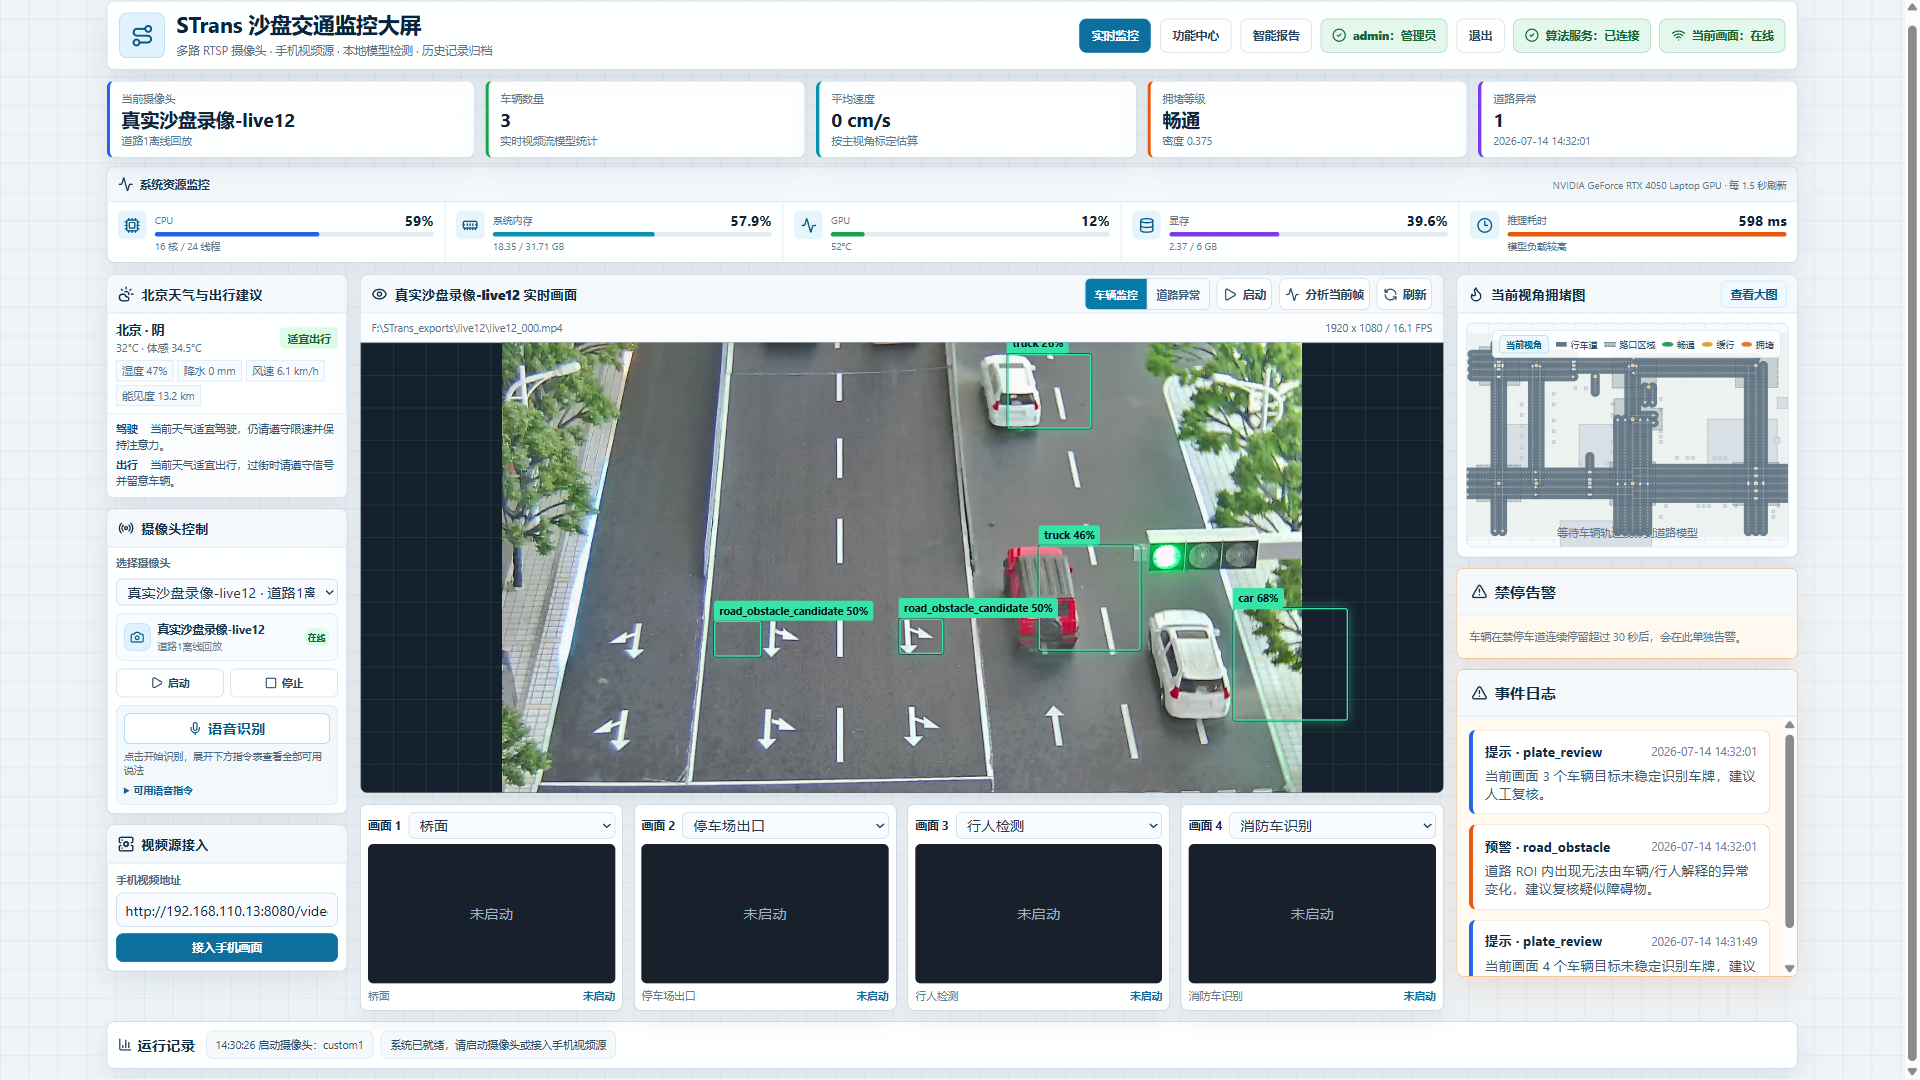
\includegraphics[keepaspectratio,alt={前端实时监控操作界面}]{assets/frontend-realtime-live12.png}}

\emph{图 6-1 前端实时监控操作界面。中央为模型标注视频，顶部为车辆、速度、拥堵和异常摘要，左侧用于视频源启停，右侧显示道路示意和事件日志。}

操作时先确认顶部``算法服务已连接''和摄像头``在线''，再观察资源监控与推理耗时是否持续稳定。截图中的道路异常候选属于需要人工复核的输出，不能仅凭候选框直接认定道路存在真实异物。

车辆监控结果经过 YOLO、ByteTrack、道路 ROI、外观过滤、轨迹稳定、HyperLPR3 和白名单决策联合生成。车牌和速度在远景、遮挡或未充分标定的摄像头上可能波动，应结合连续帧和历史记录判断。

\subsection{道路异常模式}\label{manual-ux9053ux8defux5f02ux5e38ux6a21ux5f0f}

\begin{enumerate}
\def\labelenumi{\arabic{enumi}.}
\tightlist
\item
  选择固定、画面稳定的摄像头；
\item
  将任务模式切换为``道路异常''；
\item
  等待背景和多帧候选状态建立；
\item
  查看道路异物、道路行人和可选道路破损候选；
\item
  发现告警后进入``告警处置''进行确认、解决或标记误报；
\item
  如摄像头位置、光照或场景发生明显改变，应停止并重新启动任务，必要时重置异常背景状态。
\end{enumerate}

道路异常输出定义为``候选检测 + 人工复核''。移动画面、剧烈光照、阴影、反光和道路箭头仍可能触发候选，不应将候选直接等同于真实事故或异物。

\subsection{热力图与道路状态}\label{manual-ux70edux529bux56feux4e0eux9053ux8defux72b6ux6001}

\begin{itemize}
\tightlist
\item
  已标定固定视角：车辆框底边中心通过单应矩阵映射到道路世界坐标，再计算车道、路口、禁停和拥堵；
\item
  未标定或移动视角：使用归一化画面热点，并可由 SegFormer 道路掩膜约束热点范围；
\item
  热力图表示近期活跃轨迹形成的当前状态，不是无限累计的历史轨迹图；
\item
  非参考摄像头的速度属于估计值，不能作为法定测速数据。
\end{itemize}

\section{管理与数据闭环}\label{manual-ux7ba1ux7406ux4e0eux6570ux636eux95edux73af}

\subsection{白名单管理}\label{manual-ux767dux540dux5355ux7ba1ux7406}

管理员可新增、更新和删除白名单车牌；普通用户可查看列表。车牌先做规范化和模糊匹配，再形成 \texttt{allow/\allowbreak{}deny} 软件决策。该决策用于页面显示和事件记录，当前系统没有驱动物理闸机。

白名单变更后，相关车辆的短时决策缓存会被清理。正式演示前应检查白名单内容、启用状态和 OCR 识别文本是否一致。

\subsection{历史记录}\label{manual-ux5386ux53f2ux8bb0ux5f55}

``历史记录''支持按摄像头查询，并可导出 CSV 或 JSON。记录包含模型、车辆数、密度、拥堵、检测框、事件和推理耗时等信息。管理员可删除单条或按条件清理，清理前应先备份需要保留的数据。

\subsection{告警处置与证据}\label{manual-ux544aux8b66ux5904ux7f6eux4e0eux8bc1ux636e}

\begin{enumerate}
\def\labelenumi{\arabic{enumi}.}
\tightlist
\item
  进入``告警处置''；
\item
  按状态筛选待处理事件；
\item
  查看事件类型、摄像头、时间、描述和证据；
\item
  填写处理状态、处理人和备注；
\item
  下载证据 ZIP 进行归档。
\end{enumerate}

证据包可包含事件元数据、结构化分析结果、原始帧、标注帧、清单和 SHA-256。哈希用于检查文件完整性，不代表识别结论已经人工确认。

\subsection{智能报告}\label{manual-ux667aux80fdux62a5ux544a}

管理员先在智能报告配置页填写 API 地址、模型和密钥，再基于当前检测、道路状态、天气和近期历史生成报告；普通用户可查看已归档报告。外部服务失败时应保留原始结构化数据，不能用报告生成状态替代系统识别状态。

\subsection{自适应调度}\label{manual-ux81eaux9002ux5e94ux8c03ux5ea6}

管理员可开启或关闭自适应调度。启用后，系统根据任务、静态/实时来源、CPU、内存、GPU、显存和推理耗时，在 quality、balanced、realtime、protect 和 anomaly 档位间选择模型、输入尺寸、阈值和检测间隔；关闭后进入 manual 档，使用人工配置。

资源保护档可能降低尺寸和分析频率以保持系统可用。调度只改变运行参数，不改变车辆、异常和告警的业务定义。

\section{道路建模辅助工具}\label{manual-ux9053ux8defux5efaux6a21ux8f85ux52a9ux5de5ux5177}

\subsection{使用目的}\label{manual-ux4f7fux7528ux76eeux7684}

道路建模工具用于生产二维道路拓扑、建筑物、摄像头位置和标定关系，为 RoadLogicService 的坐标映射、车道/路口归属、禁停和热力图提供配置。该工具不执行 YOLO、OCR 或异常识别。

\subsection{操作流程}\label{manual-ux64cdux4f5cux6d41ux7a0b}

\begin{enumerate}
\def\labelenumi{\arabic{enumi}.}
\tightlist
\item
  管理员打开``功能中心 → 道路建模''；
\item
  新建模型或导入已有 JSON；
\item
  设置世界尺寸、单位和网格；
\item
  创建道路节点或节点组；
\item
  按节点组连接平行车道，编辑方向、宽度和控制点；
\item
  添加建筑物和摄像头；
\item
  为摄像头添加画面点与道路实体的标定关系；
\item
  执行规范化和派生逻辑生成；
\item
  导出 \texttt{road\_\allowbreak{}logic\_\allowbreak{}modeler.\allowbreak{}v1} JSON；
\item
  人工审核、版本留存后，再交由后端道路逻辑模块使用。
\end{enumerate}

\pandocbounded{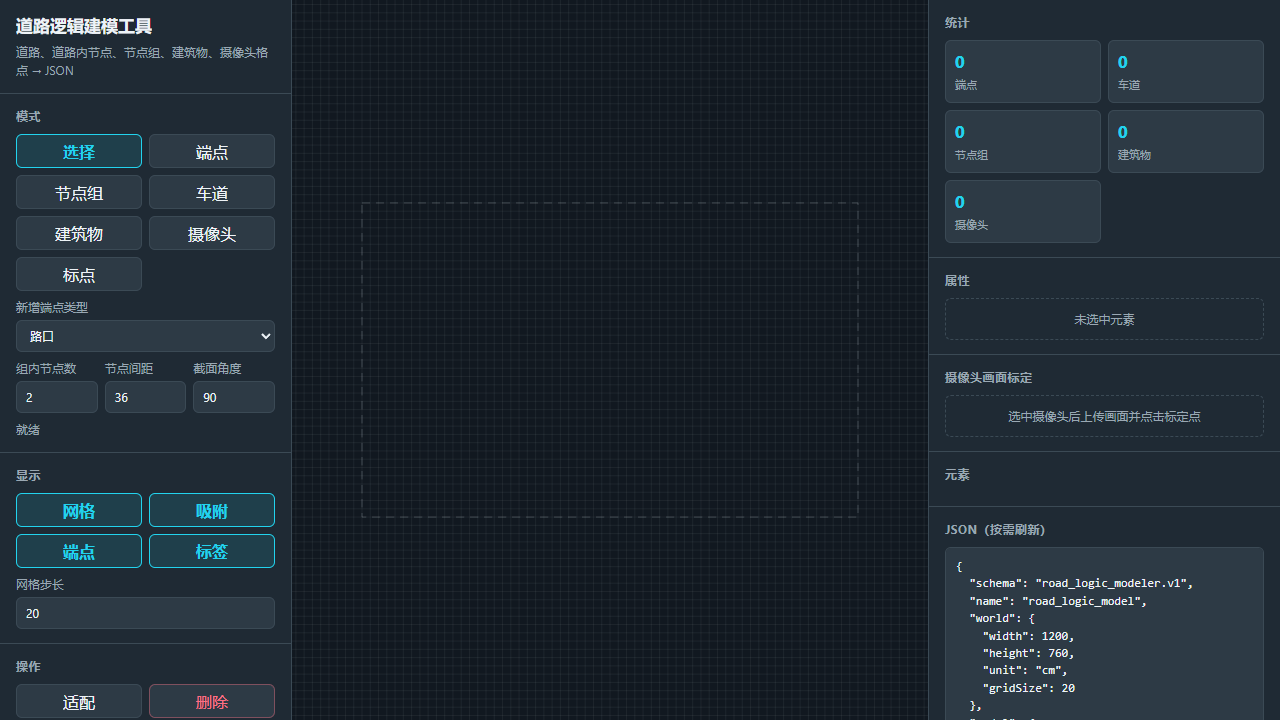
\includegraphics[keepaspectratio,alt={道路逻辑建模工具界面}]{assets/road-modeler-page.png}}

\emph{图 8-1 道路逻辑建模工具初始界面。左侧选择节点、节点组、车道、建筑物、摄像头和标点工具，中部为带网格的建模画布，右侧展示统计、属性和实时 JSON。}

建模时应先设置世界尺寸与网格，再按照``节点/节点组---车道---建筑物---摄像头---画面标定''的顺序添加对象。右侧 JSON 会随模型刷新，导出前需核对 \texttt{schema}、节点引用、车道方向和摄像头标定关系。

\subsection{发布约束}\label{manual-ux53d1ux5e03ux7ea6ux675f}

当前建模工具没有自动写回生产配置，也没有完整的``草稿---审核---发布---回滚''服务端流程。导出 JSON 必须人工检查 schema、世界尺寸、节点引用、车道方向、摄像头标定点和版本记录，不能直接覆盖正在使用的道路模型。

\section{数据、备份与证据管理}\label{manual-ux6570ux636eux5907ux4efdux4e0eux8bc1ux636eux7ba1ux7406}

\begin{itemize}
\tightlist
\item
  定期备份 SQLite 数据库、道路模型 JSON、模型权重和告警证据目录；
\item
  导出历史或证据前，记录系统版本、模型、阈值、摄像头和时间范围；
\item
  真实视频源只读使用，离线评测和截图输出写入 \texttt{output/\allowbreak{}}；
\item
  API 密钥、管理员密码和完整视频地址不得写入答辩截图、日志附件或公开仓库；
\item
  删除用户、历史、白名单或道路配置前，应先完成备份和审计确认；
\item
  数据库文件不应由多个独立后端进程同时作为同一交付实例写入。
\end{itemize}

\section{常见异常与处理}\label{manual-ux5e38ux89c1ux5f02ux5e38ux4e0eux5904ux7406}

\begin{longtable}[]{@{}
  >{\raggedright\arraybackslash}p{(\linewidth - 4\tabcolsep) * \real{0.3333}}
  >{\raggedright\arraybackslash}p{(\linewidth - 4\tabcolsep) * \real{0.3333}}
  >{\raggedright\arraybackslash}p{(\linewidth - 4\tabcolsep) * \real{0.3333}}@{}}
\toprule\noalign{}
\begin{minipage}[b]{\linewidth}\raggedright
现象
\end{minipage} & \begin{minipage}[b]{\linewidth}\raggedright
可能原因
\end{minipage} & \begin{minipage}[b]{\linewidth}\raggedright
处理方法
\end{minipage} \\
\midrule\noalign{}
\endhead
\bottomrule\noalign{}
\endlastfoot
登录页验证码不显示 & 后端未启动、网络阻塞、接口连续失败 & 检查 \texttt{/\allowbreak{}api/\allowbreak{}health}；等待 1/2/4 秒自动重试；查看浏览器网络错误 \\
前端可打开但无业务数据 & 后端地址配置错误或会话过期 & 检查 \texttt{V\allowbreak{}I\allowbreak{}T\allowbreak{}E\_\allowbreak{}\allowbreak{}A\allowbreak{}P\allowbreak{}I\_\allowbreak{}\allowbreak{}B\allowbreak{}A\allowbreak{}S\allowbreak{}E}、重新登录、确认 8000 端口 \\
视频源显示离线 & 地址错误、文件不存在、RTSP 网络异常 & 在摄像头管理执行测试；核对路径权限和网络；停止后重新启动 \\
视频有画面但无标注 & 模型未加载、权重缺失、任务模式错误 & 查看模型健康与后端日志；确认权重；检查 traffic/road\_anomaly 模式 \\
GPU 不可用 & 使用 CPU Torch、驱动或 CUDA 版本不匹配 & 在目标 Python 中检查 \texttt{torch.\allowbreak{}cuda.\allowbreak{}is\_\allowbreak{}available()}；切换已验证 CUDA 环境 \\
第一次推理明显较慢 & 模型加载、CUDA 预热、OCR 初始化 & 启动后先用固定样本预热，再开始正式演示 \\
推理延迟持续升高 & OCR 密集、多路并发、显存或内存压力 & 开启自适应调度；降低尺寸/频率；减少同时运行的流 \\
道路异常频繁误报 & 画面移动、光照变化、箭头/标线或背景未稳定 & 固定摄像头和光照；重置背景；人工标记误报；保留样本用于规则回归 \\
同类告警数量快速增长 & 实时事件缺少完整业务级冷却和生命周期合并 & 暂停异常流、按事件复核；交付版本中避免长时间无监督运行 \\
热力图位置不准 & 标定点不足、道路模型不匹配、摄像头位置改变 & 重新标定并审核 JSON；确认摄像头和模型版本对应 \\
智能报告生成失败 & API 未配置、密钥错误、外部服务不可用 & 检查脱敏配置和网络；保留历史与事件数据，稍后重试 \\
道路建模 RTSP 截帧不可用 & 本地桥接未启动或 FFmpeg 缺失 & 启动可选桥接并检查 8765；也可上传静态截图继续离线建模 \\
\end{longtable}

\section{维护与升级}\label{manual-ux7ef4ux62a4ux4e0eux5347ux7ea7}

\subsection{日常维护}\label{manual-ux65e5ux5e38ux7ef4ux62a4}

\begin{enumerate}
\def\labelenumi{\arabic{enumi}.}
\tightlist
\item
  每次演示前检查后端、前端、GPU、模型健康、磁盘空间和摄像头连通性；
\item
  使用固定视频执行短回归，核对车辆框、历史写入、告警和热力图；
\item
  定期清理无价值测试历史和重复告警，但保留缺陷复现样本；
\item
  监控 CPU、内存、GPU、显存和推理耗时，记录异常峰值；
\item
  对白名单、用户、摄像头和道路模型的变更保留审计和版本记录。
\end{enumerate}

\subsection{版本升级}\label{manual-ux7248ux672cux5347ux7ea7}

升级 Python、PyTorch、CUDA、OpenCV、Ultralytics、HyperLPR3 或 Transformers 后，应至少执行：

\begin{Verbatim}[breaklines=true,breakanywhere=true,fontsize=\small,frame=single,framesep=2mm,rulecolor=\color{STransLine}]
cd backend
python -m pytest tests -q -W error::ResourceWarning

cd ..\frontend
pnpm test
pnpm build

cd ..
python -m pytest tools\road_logic_modeler\tests -q
\end{Verbatim}

还应使用固定真实视频复测推理耗时和代表性画面。自动化全通过只能证明已有用例未回归，不能替代真实数据质量评估。

\section{已知限制}\label{manual-ux5df2ux77e5ux9650ux5236}

\begin{enumerate}
\def\labelenumi{\arabic{enumi}.}
\tightlist
\item
  F 盘真实视频尚无完整人工框、车牌和事件真值，当前不能给出 Precision、Recall、F1 或整牌准确率；
\item
  道路箭头等高对比标线可能触发道路异常候选；
\item
  同类实时事件仍可能逐帧写入，事件级冷却、合并和生命周期需要继续完善；
\item
  非参考摄像头速度为估计值，摄像头变化后必须重新标定；
\item
  极远景、严重遮挡和极小车牌存在漏检或 OCR 波动；
\item
  道路破损识别依赖可选权重和样本质量；
\item
  尚未完成独立 FastAPI 权限/错误码矩阵、断流恢复和 30--60 分钟长稳测试；
\item
  智能报告依赖外部服务，其生成质量不属于本地算法测试结论；
\item
  道路建模输出仍需人工审核后发布；
\item
  当前成果是二维道路模型与视觉分析平台，不是完整三维数字孪生系统。
\end{enumerate}

\section{交付验收检查表}\label{manual-ux4ea4ux4ed8ux9a8cux6536ux68c0ux67e5ux8868}

\begin{itemize}
\tightlist
\item[$\square$]
  后端健康接口可访问；
\item[$\square$]
  前端登录、验证码和双角色权限正确；
\item[$\square$]
  至少一路固定视频可启动并显示原始/标注画面；
\item[$\square$]
  CUDA 环境、模型名称、阈值、输入尺寸和推理耗时已记录；
\item[$\square$]
  车辆监控与道路异常模式互不污染；
\item[$\square$]
  历史记录、告警处置和证据导出可用；
\item[$\square$]
  白名单、摄像头、模型和调度管理可用；
\item[$\square$]
  道路建模页面与 \texttt{road\_\allowbreak{}logic\_\allowbreak{}modeler.\allowbreak{}v1} 导出可用；
\item[$\square$]
  已知误报、事件重复和无完整真值限制已写入报告；
\item[$\square$]
  SQLite、道路模型和证据目录已完成交付备份。
\end{itemize}
